\section{Started again}

9 déc. 2011

\begin{multicols}{2}

Hello everybody, let's get restarted !!!

Certain le savent, je suis reparti pour une boucle de quelque semaines direction les Philippines où je vais essayer de découvrir certaines îles de cet immense archipel, puis je retournerai à Bali pour revoir mon pote Sales qui est là bas. On essaiera d'aller dans des endroits que je n'ai pas encore vu et mon trip serat d'aller pêcher avec lui au petit matin. Florian me rejoindra vers fin decembre pour passer le réveillon et bouger encore quelque jours puis viendra la dernière escale du voyage (enfin.. ça va peut être changer d'ici là). Nous devions normalement terminer par le Calédonie où on devait rejoindre Patrick et son super Bateau (souvenez vous le passage de l'équateur en 2008.. c'était lui). Ca c'était le plan jusqau'à lundi dernier, mais l'eau salée est venu et le moteur de la Tiare Moana a succombé. N'ayant plus de bateau pour les mois qui viennent Patrick ne reste plus en Calédonie pour nous accueillir et nous ne pouvons donc plus y aller.

Changement de plan donc, heureusement possible car nos billets n'étaient pas encore pris pour la Calédonie. Nous irons donc au Viêtnam.. C'est une destination que je n'avais pas pu visiter il y a quatre ans et j'ai vraiement envie d'aller voir cette fois-ci. On ajoutera peut être une dernière escale avant de rentrer fin janvier.. mais comme c'est pas certain on en parlera plus tard..

Voici une carte pour situer tout ça, pour l'heure je suis à Manille mais je n'ai pas encore vu grand chose donc je ne vais pas m'étaler, j'en parlerai sûrement vers la fin de ma boucle aux Philippines, d'ici là je vais essayer d'aller demain vers Palawan siroter un moijto ou deux sur la plage et vers d'autres encroits dont je ne connais pas encore les noms..

%\hspace*{-0.65cm}
%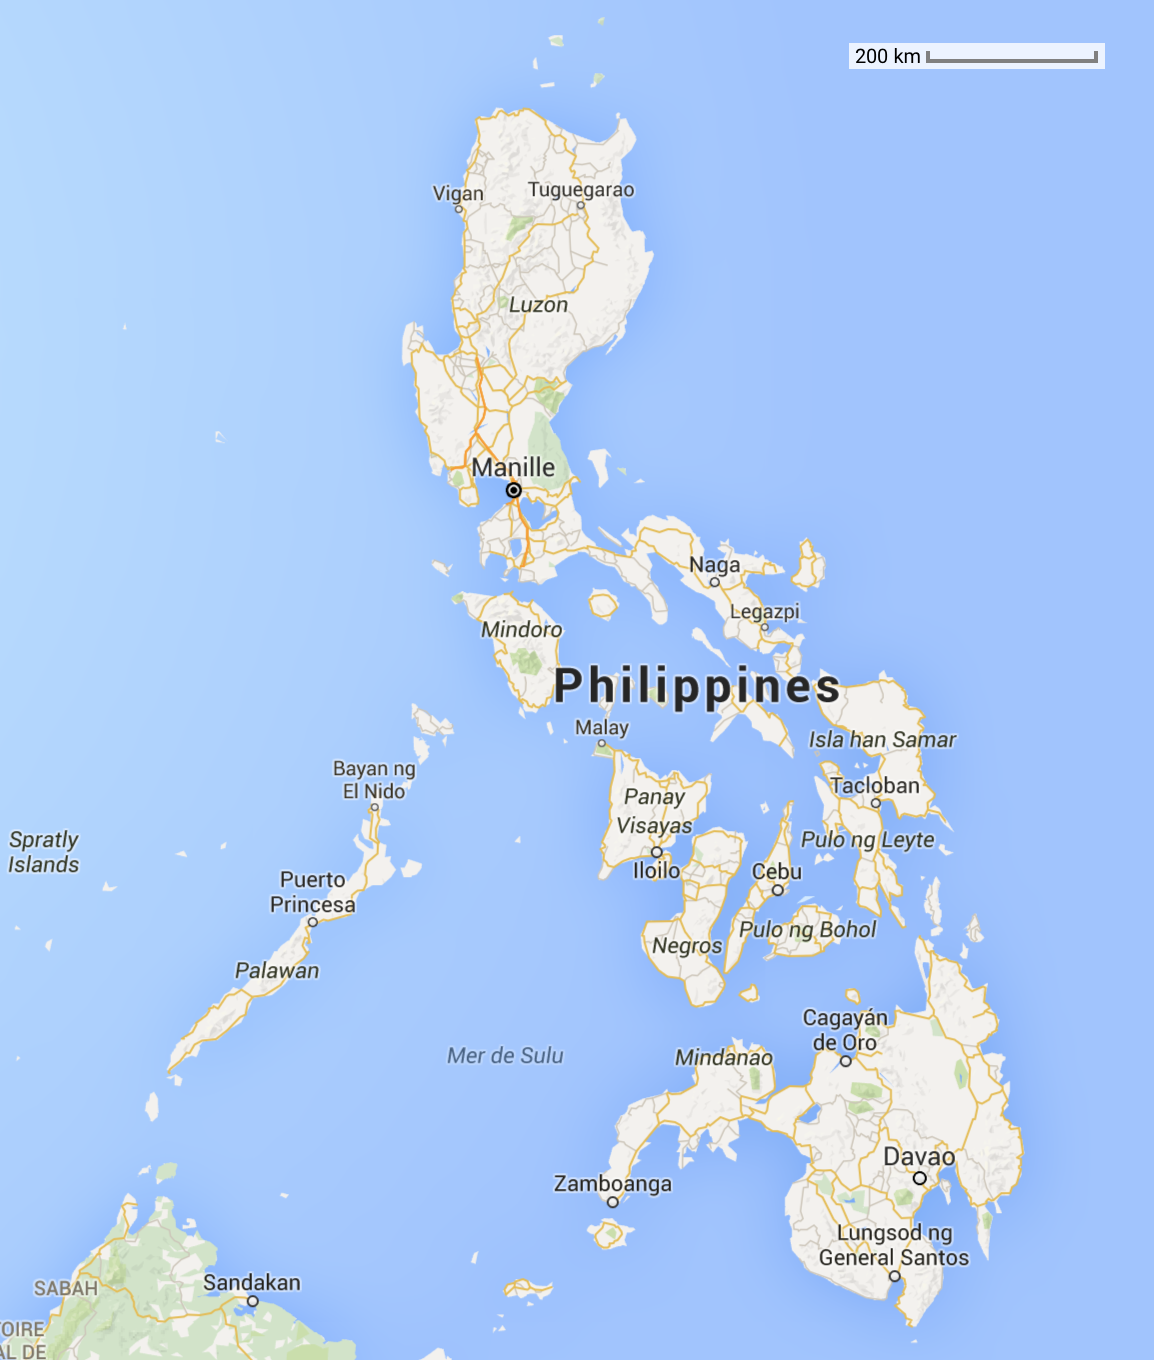
\includegraphics[width=4.8cm]{articles/Started-again/philippines.png}
%Carte des Philippines.

Ah oui j'oubliais, vous venez sur ce blog a vos risques et périls, je ne pourrais être tenu pour responsable d'une quelconque envie de voyage même si la propagation de ce virus est grandement encouragée par la maison. Maintenant que c'est dit, à bientôt :)

\end{multicols}

\bigskip
\textbf{\textsc{Commentaires}}

\medskip
Dova a écrit le 13 déc. 2011 :
\begin{displayquote}
Coucou Loulou,

J'espère que ton début de séjour aux Philippines se passe bien. 
Profites pour nous et n'oublies pas les photos... afin de rêver du haut de notre montagne ;)...

Gros bisous
\end{displayquote}

\medskip
El Duderino a écrit le 15 déc. 2011 :
\begin{displayquote}
Profites bien de ces mojitos et bazardes quelques photos. Bref, fais nous rever!
Buen viaje amigo, que le vaya bien...
\end{displayquote}


